\documentclass[c]{beamer}
\usepackage[english]{LNTbeamer}
%\usepackage[german]{LNTbeamer} % For German
%\usepackage[english,ocsgroup]{LNTbeamer} %For English and the OCSGroup


% For Documentation on the Beamer class in General please go to
% www.ctan.org/tex-archive/macros/latex/contrib/beamer/doc/beameruserguide.pdf

\title[Vector Network Coding Gap Sizes for the Generalized Combination Network]{Vector Network Coding Gap Sizes for the Generalized Combination Network}
\author[Ha Nguyen]{Ha Nguyen\\ {\footnotesize \hspace{1mm} ha.nguyen@tum.de} }
\date{\today}

% LYX
\usepackage{array}


\begin{document}

%------------------------------------------------------------------------------------------------------------------------------------------
%												TITLE (Automatisch)
%------------------------------------------------------------------------------------------------------------------------------------------
\begin{frame}
	\titlepage
\end{frame}

%------------------------------------------------------------------------------------------------------------------------------------------
%												OUTLINE
%------------------------------------------------------------------------------------------------------------------------------------------
\section*{Outline}
\begin{frame}
	\frametitle{Outline}
	\tableofcontents
\end{frame}


\section{Motivation}
%------------------------------------------------------------------------------------------------------------------------------------------
%												MOTIVATION
%------------------------------------------------------------------------------------------------------------------------------------------
\begin{frame}[c]
\frametitle{Motivation}
	\begin{itemize}%[<1->]
		\item General vector solutions for the Generalized Combination Network was not found. 

	\begin{example}[A multicast network with 3 messages]
		\begin{figure}

		\caption{Vector Network Coding Outperforms Scalar Network Coding}

		\centering{}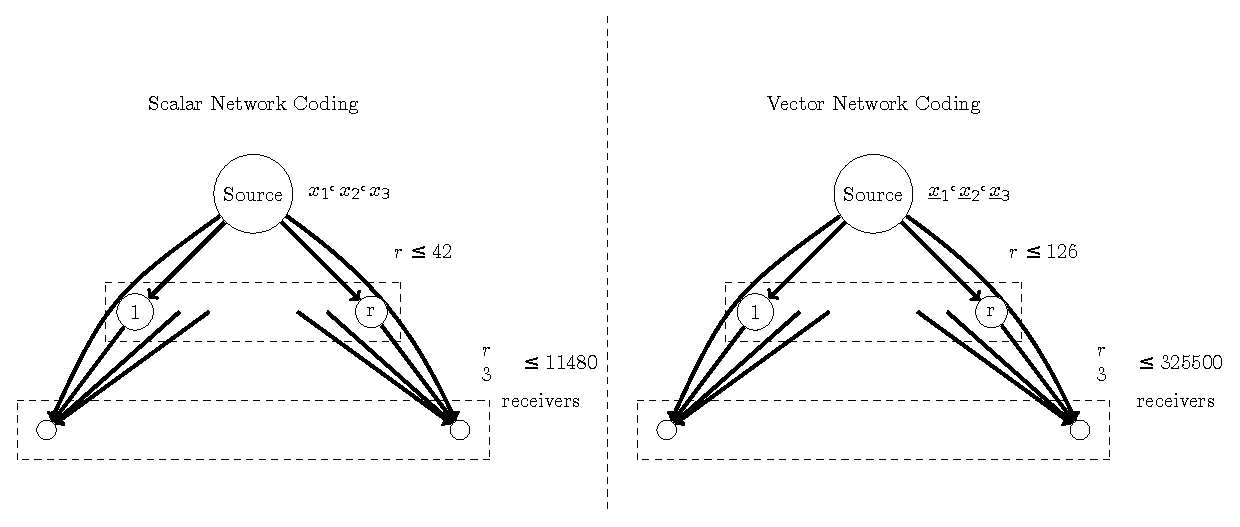
\includegraphics[width=0.6\paperwidth]{../figures/slide_scalar_vector_nc}
		\end{figure}
	\end{example}

		\item[$\Longrightarrow$] Vector Network Coding provides a higher number of receivers.
	\end{itemize}
\end{frame}


%------------------------------------------------------------------------------------------------------------------------------------------
%												MOTIVATION
%------------------------------------------------------------------------------------------------------------------------------------------
%\begin{frame}[c]
%\frametitle{Motivation continued}

	
%\end{frame}



%------------------------------------------------------------------------------------------------------------------------------------------
%            What is Network Coding? - Initial Idea
%------------------------------------------------------------------------------------------------------------------------------------------

\section{What is Network Coding?}
\subsection{Initial Idea}
\begin{frame}[c]
\frametitle{Initial Idea}

	\begin{itemize}
		\item \textit{Network coding} was first introduced in Ahlswede et al.'s seminal paper \cite{Ahlswede:2000} with the well-known butterfly network.
			\begin{figure}[H]
			\caption{The butterfly network \label{fig:The-butterfly-network}}
			
			\centering{}\includegraphics[width=0.5\paperwidth]{../figures/ahlswede_butterfly_network}
			\end{figure}
		\item[$\Longrightarrow$] Network coding gives a potential gain in throughput by communicating more information with fewer packet transmissions compared to the routing method.
	\end{itemize}

\end{frame}

%------------------------------------------------------------------------------------------------------------------------------------------
%		What is Network Coding? - Network as Matrix Channel
%------------------------------------------------------------------------------------------------------------------------------------------
\subsection{Network as Matrix Channel}
\begin{frame}[c]
\frametitle{Network as Matrix Channel}
	\begin{itemize}
		\item In our study, we formulate networks as matrix channels.
			\begin{equation}
			\begin{array}{c|c}
			Scalar & Vector\\
			\underset{\ensuremath{\mathbb{F}}_{q_{\mathrm{s}}}^{s}}{\underbrace{\left[\begin{array}{c}
			y_{j_{1}}\\
			\vdots\\
			y_{j_{s}}
			\end{array}\right]}}=\underset{\ensuremath{\mathbb{F}}_{q_{\mathrm{s}}}^{s\times h}}{\underbrace{\boldsymbol{A}_{j}}}\cdot\underset{\ensuremath{\mathbb{F}}_{q_{s}}^{h}}{\underbrace{\left[\begin{array}{c}
			x_{1}\\
			\vdots\\
			x_{h}
			\end{array}\right]}} & \underset{\ensuremath{\mathbb{F}}_{q}^{st}}{\underbrace{\left[\begin{array}{c}
			\boldsymbol{y}_{j_{1}}\\
			\vdots\\
			\boldsymbol{y}_{j_{s}}
			\end{array}\right]}}=\underset{\ensuremath{\mathbb{F}}_{q}^{st\times th}}{\underbrace{\boldsymbol{A}_{j}}}\cdot\underset{\ensuremath{\mathbb{F}}_{q}^{th}}{\underbrace{\left[\begin{array}{c}
			\boldsymbol{x}_{1}\\
			\vdots\\
			\boldsymbol{x}_{h}
			\end{array}\right]}}
			\end{array}\label{eq:linear_system}
			\end{equation}

			\[
			\begin{array}{c|c}
			Scalar & Vector\\
			\boldsymbol{A}_{j}=\left[\begin{array}{c}
			\boldsymbol{a}_{j_{1}}\\
			\vdots\\
			\boldsymbol{a}_{j_{\alpha\ell}}\\
			\vdots\\
			\boldsymbol{a}_{j_{\alpha\ell+\epsilon}}
			\end{array}\right] & \boldsymbol{A}_{j}=\left[\begin{array}{c}
			\boldsymbol{A}_{j_{1}}\\
			\vdots\\
			\boldsymbol{A}_{j_{\alpha l}}\\
			\vdots\\
			\boldsymbol{A}_{j_{\alpha l+\epsilon}}
			\end{array}\right]
			\end{array}
			\]		
	\end{itemize}	
\end{frame}

%------------------------------------------------------------------------------------------------------------------------------------------
%            What is Network Coding? - Our Choice of Network
%------------------------------------------------------------------------------------------------------------------------------------------
\subsection{Generalized Combination Network}
\begin{frame}[c]
\frametitle{Generalized Combination Network}

	\begin{itemize}
		\item We choose to use the Generalized Combination Network to analyze its network coding problems. The well-known butterfly network is isomorphic to $\mathcal{N}_{h,r=3,s=2}$, if we consider it as
an undirected network \cite{Maheshwar:2012}
			\begin{figure}[H]
			\caption{The butterfly network is represented as a combination network \label{fig:butterfly_nw_cn}}
			
			\centering{}\includegraphics[width=0.5\paperwidth]{../figures/ahlswede_butterfly_network_CN}
			\end{figure}
	\end{itemize}

\end{frame}

%------------------------------------------------------------------------------------------------------------------------------------------
%            What is Network Coding? - Our Choice of Network
%------------------------------------------------------------------------------------------------------------------------------------------
\begin{frame}[c]
\frametitle{Generalized Combination Network [cont.]}

	\begin{itemize}
		\item A generalized combination network $(\epsilon,\ell)-\mathcal{N}_{h,r,s}$ consists of 3 components over 3 layers from top to bottom: “Source” in the first layer, “Intermediate Nodes” in the middle layer, and “Receiver” in the third layer.
			\begin{figure}[H]
			\caption{The generalized network $(\epsilon,\ell)-\mathcal{N}_{h,r,s}$\label{fig:The-generalized-network}}
			
			\centering{}\includegraphics[width=0.5\paperwidth]{../figures/generalized_combination_nw}
			\end{figure}
	\end{itemize}

\end{frame}

%------------------------------------------------------------------------------------------------------------------------------------------
%            What is Network Coding? - Our Choice of Network
%------------------------------------------------------------------------------------------------------------------------------------------
\begin{frame}[c]
\frametitle{Generalized Combination Network [cont.]}

\begin{table}[H]
\caption{Parameters of network coding \label{tab:Parameters-of-network}}

\centering{}%
\begin{tabular}{c|>{\centering}p{0.60\paperwidth}}
$h$ & The number of source messages\tabularnewline
\hline 
$r$ & The number of nodes in the middle layer\tabularnewline
\hline 
$\left(\begin{array}{c}
r\\
\alpha
\end{array}\right)$ & The number of receivers\tabularnewline
\hline 
$\ell$ & The source connects to each node by $\ell$ parallel links, and each
node also connects to one receiver by $\ell$ parallel links\tabularnewline
\hline 
$\alpha$ & A receiver is connected by any $\alpha$ nodes in the middle layer\tabularnewline
\hline 
$\epsilon$ & The source additionally connects to each receiver by $\epsilon$ direct
parallel links\tabularnewline
\hline 
$s$ & Each receiver is connected by $s$ links in total, with $s=\alpha\ell+\epsilon$.\tabularnewline
\end{tabular}
\end{table}


\end{frame}

%%%%%%%%%%%%%%%%%%%%%%%%%%%
\subsection{Introduction of Gap}
\begin{frame}[c]
\frametitle{Introduction of Gap}

	\begin{itemize}
		\item The gap represents the difference between the smallest field (alphabet) size for which a scalar linear solution exists and the smallest alphatbet size for which we can construct a vector solution.	
		\item $r_{max,vector}\geq f_{1}(q,t,\alpha,h)$, with $f_{1}:\mathbb{Z}\mapsto\mathbb{Z}$
		\item $r_{scalar}\leq f_{2}\left(q_{\mathrm{s}}\right)$,
with $f_{2}:\mathbb{Z}\mapsto\mathbb{Z}$
		\item $r_{max,scalar}=f_{2}\left(q_{\mathrm{s}}\right)=f_{1}(q,t,\alpha,h)=min\left\{r_{max,vector}\right\}$.
Finally, we calculate the gap by $g=q_{\mathrm{s}}-q_{v}=q_{\mathrm{s}}-q^{t}.$
		
	\end{itemize}

\end{frame}

%%%%%%%%%%%
\begin{frame}[c]
\frametitle{Introduction of Gap [cont.]}
		\begin{table}
		
		\caption{New gap found in this study \label{tab:New-gap-found}}
		
		\begin{centering}
		\begin{tabular}{|>{\centering}p{0.30\paperwidth}|>{\centering}p{0.2\paperwidth}|>{\centering}p{0.3\paperwidth}|}
		\hline 
		\centering{}Network & \centering{}Gap Bounds for a specific vector solution \cite{Wachter-Zeh:2018} & \centering{}This study proves an existence of these gaps\tabularnewline
		\hline 
		\hline 
		\centering{}$\left(\epsilon=0,\ell=1\right)-\mathcal{N}_{h,r,s}$ & \centering{}N/A & \centering{}N/A\tabularnewline
		\hline 
		\centering{}$\left(\epsilon\geq1,\ell=1\right)-\mathcal{N}_{h,r,s}$ & \centering{}Unknown & \centering{}$q^{\frac{\alpha-h+1}{\left(\alpha-1\right)\left(\alpha-h+2\right)\left(h-2\right)}t^{2}+\mathcal{O}(t)}$
		({*})\tabularnewline
		\hline 
		\begin{centering}
		$(\epsilon=1,\ell\geq2)-$
		\par\end{centering}
		$\mathcal{N}_{h=2\ell,r,s=2\ell+1}$ & \centering{}$q^{t^{2}/2+\mathcal{O}\left(t\right)}$ & \centering{}$q^{t^{2}/l+\mathcal{O}\left(t\right)}$\tabularnewline
		\hline 
		\begin{centering}
		$\left(\epsilon=\ell-1,\ell\right)-$
		\par\end{centering}
		$\mathcal{N}_{h=2\ell,r,s=3\ell-1}$ & \centering{}$q^{t^{2}/2+\mathcal{O}\left(t\right)}$ & \centering{}N/A\tabularnewline
		\hline 
		\end{tabular}
		\par\end{centering}
		\begin{centering}
		({*}): We only consider the $\left(\epsilon=1,\ell=1\right)-\mathcal{N}_{h,r,s}$
		network.
		\par\end{centering}
		\end{table}
\end{frame}

%------------------------------------------------------------------------------------------------------------------------------------------
%            Combinatorial Results
%------------------------------------------------------------------------------------------------------------------------------------------

\section{Combinatorial Results}
\subsection{$\left(\epsilon=1,\ell=1\right)-\mathcal{N}_{h=3,r,s=4}$ Network}
\begin{frame}[c]
\frametitle{$\left(\epsilon=1,\ell=1\right)-\mathcal{N}_{h=3,r,s=4}$ Network}
	\begin{lemma}[Symmetric Lov\'asz local lemma (LLL) \cite{Schwarz:2013}]
 A set of events $\mathcal{E}_{i}$, with $i=1,\ldots,n$, such that
each event occurs with probability at most $p$. If each event is
independent of all others except for at most $d$ of them and $4dp\leq1$,
then: $Pr\left[\stackrel[i=1]{n}{\bigcap}\overline{\mathcal{E}}_{i}\right]>0$.
\label{thm:LLL}
	\end{lemma}
\end{frame}

%%%%%%%%%%%
\begin{frame}[c]
\frametitle{$\left(\epsilon=1,\ell=1\right)-\mathcal{N}_{h=3,r,s=4}$ Network [cont.]}

	\begin{lemma}
\label{lem:prob_p_LLL_formula}{\footnotesize{} Let $Pr\left[\mathcal{E}_{i}\right]=Pr\left[rk\left[\begin{array}{c}
\boldsymbol{A}_{j}^{\left(r_{1}\right)}\\
\boldsymbol{A}_{j}^{\left(r_{1}\right)}\\
\boldsymbol{A}_{j}^{\left(r_{3}\right)}
\end{array}\right]<2t\right]\leq p,\forall1\leq r_{1}<r_{2}<r_{3}\leq r$, and $\boldsymbol{A}_{j}^{\left(r_{1}\right)},\ldots,\boldsymbol{A}_{j}^{\left(r_{3}\right)}\in\ensuremath{\mathbb{F}}_{q}^{t\times3t}$,
then, 
\[
p\leq\Theta\left(q^{-t^{2}-2t-1}\right),\forall t\geq2.
\]
}{\footnotesize\par}
	\end{lemma}
	\begin{lemma}
{\footnotesize{} Let $Pr\left[\mathcal{E}_{i}\right]=Pr\left[rk\left[\begin{array}{c}
\boldsymbol{A}_{j}^{\left(r_{1}\right)}\\
\boldsymbol{A}_{j}^{\left(r_{1}\right)}\\
\boldsymbol{A}_{j}^{\left(r_{3}\right)}
\end{array}\right]<2t\right]\leq p,\forall1\leq r_{1}<r_{2}<r_{3}\leq r$ with $\boldsymbol{A}_{j}^{\left(r_{1}\right)},\ldots,\boldsymbol{A}_{j}^{\left(r_{3}\right)}\in\ensuremath{\mathbb{F}}_{q}^{t\times3t}$,
and each event $\mathcal{E}_{i}$ is independent of all others except
for at most $d$ of them, then $d\leq\frac{3}{2}r^{2}$. \label{lem:dependecy_d_LLL}
}{\footnotesize\par}
	\end{lemma}
\end{frame}

%%%%%%%%%%%
\begin{frame}[c]
\frametitle{$\left(\epsilon=1,\ell=1\right)-\mathcal{N}_{h=3,r,s=4}$ Network [cont.]}

	\begin{theorem}
If $r\leq\Omega\left(q^{t^{2}/2+\mathcal{O}\left(t\right)}\right)$,
then there exists a vector solution for the $\left(\epsilon=1,l=1\right)-\mathcal{N}_{h=3,r,s=4}$
network. \label{theo:r_for_vector_sol_e1l1h3rs4}
	\end{theorem}
	
	\begin{corollary}
	The $\left(\epsilon=1,\ell=1\right)-\mathcal{N}_{h=3,r,s=4}$ network
	has a vector solution with a gap $q^{t^{2}/4+\mathcal{O}(t)}$.
	\end{corollary}
\end{frame}

%%%%%%%%%%%%%%%%%%%%%%%%%%%%%%%%%%%%%%
\subsection{$\left(\epsilon=1,\ell=1\right)-\mathcal{N}_{h,r,s}$ Network}
\begin{frame}[c]
\frametitle{$\left(\epsilon=1,\ell=1\right)-\mathcal{N}_{h,r,s}$ Network}

	\begin{itemize}
		\item Item 1
		\item Item 2
		\item Item 3
	\end{itemize}


\end{frame}

%%%%%%%%%%%%%%%%%%%%%%%%%%%%%%%%%%%%%%
\subsection{$\left(\epsilon=1,\ell\protect\geq2\right)-\mathcal{N}_{h=2\ell,r,s=2\ell+1}$
Network}
\begin{frame}[c]
\frametitle{$\left(\epsilon=1,\ell\protect\geq2\right)-\mathcal{N}_{h=2\ell,r,s=2\ell+1}$
Network}

	\begin{itemize}
		\item Item 1
		\item Item 2
		\item Item 3
	\end{itemize}
\end{frame}

%------------------------------------------------------------------------------------------------------------------------------------------
%            Computational Results
%------------------------------------------------------------------------------------------------------------------------------------------

\section{Computational Results}
\subsection{$\left(\epsilon=1,\ell=1\right)-\mathcal{N}_{h=3,r,s=4}$ Network}
\begin{frame}[c]
\frametitle{$\left(\epsilon=1,\ell=1\right)-\mathcal{N}_{h=3,r,s=4}$ Network}
\begin{table}[H]
\caption{$r$ over variations of t\label{tab:r_over_t}}

\begin{centering}
\begin{tabular}{|c|c|c|}
\hline 
t & Scalar Solution & Vector Solution\tabularnewline
\hline 
\hline 
1 & $r_{scalar}\leq14$ & $r_{vector}\geq3$\tabularnewline
\hline 
2 & $r_{scalar}\leq42$ & $r_{vector}\geq7\,\left(67^{*},\,89^{**}\right)$\tabularnewline
\hline 
3 & $r_{scalar}\leq146$ & $r_{vector}\geq62\,\left(166^{*}\right)$ \tabularnewline
\hline 
4 & $r_{scalar}\leq546$ & $r_{vector}\geq1317$\tabularnewline
\hline 
5 & $r_{scalar}\leq2114$ & $r_{vector}\geq58472$\tabularnewline
\hline 
6 & $r_{scalar}\leq8322$ & $r_{vector}>10^{6}$\tabularnewline
\hline 
\end{tabular}
\par\end{centering}
{*}, {*}{*}: computational results in construction 1 and construction
2 respectively
\end{table}
\end{frame}

%------------------------------------------------------------------------------------------------------------------------------------------
%												Conclusions
%------------------------------------------------------------------------------------------------------------------------------------------
\section{Conclusions}
\begin{frame}[c]
\frametitle{Conclusions and Outlook}
	
	\begin{itemize}
		\item If $r\leq\Omega\left(q^{t^{2}/2+\mathcal{O}\left(t\right)}\right)$,
there always exists a vector solution for the $\left(\epsilon=1,\ell=1\right)-\mathcal{N}_{h=3,r,s=4}$
network.
		\item The
general gap $g=q^{t^{2}/4+\mathcal{O}(t)}$ can be achieved for the $\left(\epsilon=1,\ell=1\right)-\mathcal{N}_{h=3,r,s=4}$
network
		\item For the $\left(\epsilon=1,\ell=1\right)-\mathcal{N}_{h=3,r,s=4}$
network. Similarly we derived the gaps for the $\left(\epsilon=1,\ell=1\right)-\mathcal{N}_{h,r,s}$
network and the $\left(\epsilon=1,\ell>1\right)-\mathcal{N}_{h=2\ell,r,s=2\ell+1}$
network, respectively with $g=q^{\frac{\alpha-h+1}{\left(\alpha-1\right)\left(\alpha-h+2\right)\left(h-2\right)}t^{2}+\mathcal{O}(t)}$
and $g=q^{t^{2}/2\ell+\mathcal{O}(t)}$.
		\item An improved bound $89\leq\mathcal{A}_{2}\left(6,4,3;2\right)\leq126$.
		\item A new bound $166\leq\mathcal{A}_{2}\left(9,6,3;2\right)\leq537$.
	\end{itemize}

\end{frame}


%------------------------------------------------------------------------------------------------------------------------------------------
%												References
%------------------------------------------------------------------------------------------------------------------------------------------

\section*{References}
\begin{frame}[b]
% 	\frametitle{References}

	\vskip15pt
	\begin{beamercolorbox}[center,rounded=true,sep=2mm,shadow=true]{block title}
		\Large Thank you! Questions?	
	\end{beamercolorbox}

	
	\vskip25pt
	\structure{\large References:}
	% Use IEEE DIN 1505 style for bibliography / Literaturverzeichnisses
	\bibliographystyle{IEEEtran}
	%\nocite{*}              % Include all references without checking / Alle References immer aufführen
	\bibliography{../refs/final_ref_bib}
	\vskip3pt
\end{frame}

\end{document}